% ============PREAMBLE SECTION==========================================
%+++++++++++++++++++++++++++++++++++++++++++++++++++++++++++++++++++++++
\documentclass[12pt]{article}
\usepackage{geometry}                % See geometry.pdf to learn the layout options. There are lots.
\geometry{letterpaper}                   % ... or a4paper or a5paper or ... 
%\geometry{landscape}                % Activate for for rotated page geometry
\usepackage[parfill]{parskip}    % Activate to begin paragraphs with an empty line rather than an indent
\usepackage{daves,fancyhdr,natbib,graphicx,dcolumn,amsmath,lastpage,url}
\usepackage{amsmath,amssymb,epstopdf,longtable}


% other
\usepackage{paralist}  % need to modify standard enumerate blocks
%=========Longtable environment
\usepackage{setspace}                % allow single and double space environment
\usepackage{longtable}                % allow table to span multiple pages
\usepackage{caption}                    % consistent caption package
\usepackage{url}					% Ubiquitious url formatting package
%===========

\DeclareGraphicsRule{.tif}{png}{.png}{`convert #1 `dirname #1`/`basename #1 .tif`.png}
\pagestyle{fancy}
\lhead{Student Name: \_\_\_\_\_\_\_\_\_\_\_\_\_\_\_\_\_\_\_\_\_\_\_\_\_\_\_\_\_\_\_\_\_\_\_\_\_\_\_\_\_\_\_\_\_ }
\rhead{FALL 2024}
\lfoot{CE 5364 Groundwater Transport }
\cfoot{EXAM 1}
\rfoot{Page \thepage\ of \pageref{LastPage}}
\renewcommand\headrulewidth{0pt}
%++++++++++++++++++++++++++++++++++++++++++++++++++++++++++++++++++++++++++
%============================================================================
\begin{document}

\begingroup
\begin{centering}
\textbf{CE 5364 Groundwater Transport Phenomena } \\
\textbf{Exam 1 (Alternate) , Fall 2024}\\
\end{centering}
~\\
Students should write their name on \textbf{all sheets of paper}.  \newline 
Students are permitted to use the internet to help answer questions.  \newline 
Students are permitted to use their own notes and the textbook.\newline 
Students are \textbf{forbidden} to \textbf{communicate with other people} during the examination.
\endgroup

\begin{enumerate}
\item Provide short answers to the following questions:
\begin{enumerate}[a)]
\item What is an adsorbtion isotherm?
~\newline
~\newline
~\newline
~\newline
~\newline
\item Why is it important in contaminant hydrology?
~\newline 
~\newline
~\newline
~\newline
~\newline
~\newline
\item  What is the advection-dispersion equation?
~\newline
~\newline
~\newline
~\newline
~\newline
~\newline
\item Why is it important in contaminant hydrology?
~\newline
~\newline
~\newline
~\newline
~\newline
~\newline
\end{enumerate}
\clearpage
%%%%%%%%%%%%%%%%%%%%%%%%%%%%%%%%%%%%%%%%%%%%%%%%%%%%%%%%%%%%%%%%%%%%%%%
\item  Consider the concentration profiles in Figure \ref{fig:profile1}.  The elapsed time, 10 days, is the time since the injection of a constituient bolous.  Assuming the porosity is 0.50 and the initial mass of constituient is 200 mg.
\begin{figure}[h!] %  figure placement: here, top, bottom, or page
   \centering
   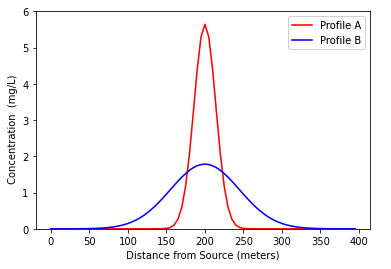
\includegraphics[width=4in]{profile1.png} 
   \caption{Concentration profile(s)}
   \label{fig:profile1}
\end{figure}
Determine:
\begin{enumerate}
\item The profile (A) or (B) that indicates greater dispersive behavior.
\item The model that describes the type of transport indicated by the profile.
\item The pore velocity and apparent dispersion for each profile.
\end{enumerate}
\clearpage
Continued (show work here)
\clearpage
\item  Consider the concentration histories in Figure \ref{fig:history1}.  The elapsed time is the time since the release of the constituients. The observation location is 100 meters away from the source zone. 
\begin{figure}[h!] %  figure placement: here, top, bottom, or page
   \centering
   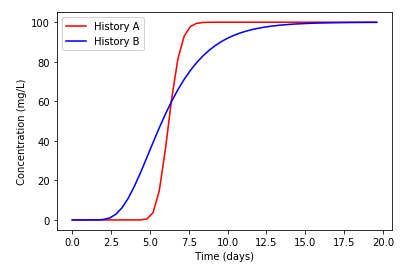
\includegraphics[width=4in]{history1.png} 
   \caption{Concentration histories}
   \label{fig:history1}
\end{figure}
Determine:
\begin{enumerate}
\item The history (A) or (B) that indicates greater dispersive behavior.
\item The model that describes the type of transport indicated by the history.
\item The pore velocity and apparent dispersion for each history.
\end{enumerate}
\clearpage
Continued (show work here)
\clearpage %%%%%%%%%%%%%%%%%%%%%
\item Assume that one-dimensional transport tools are adequate to simulate the transport of a contaminant through an aquifer depicted in Figure \ref{fig:aquifer1}
\begin{figure}[h!] %  figure placement: here, top, bottom, or page
   \centering
   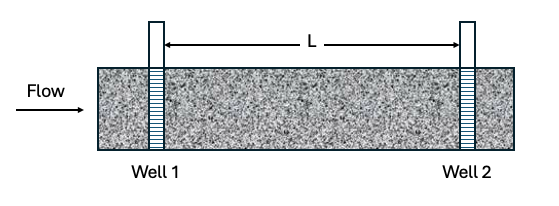
\includegraphics[width=4in]{aquifer1.png} 
   \caption{Aquifer Schematic}
   \label{fig:aquifer1}
\end{figure}
For each situation described below, write the governing equation(s) (not the solutions) describing the transport (and any reactions). Sketch the expected concentration history at Well 2 for the history given at Well 1.
\begin{enumerate}
\item Constant source; no dispersion, reactions, or decay. ~\\~\\
%\begin{figure}[h!] %  figure placement: here, top, bottom, or page
%\centering
\begin{center}
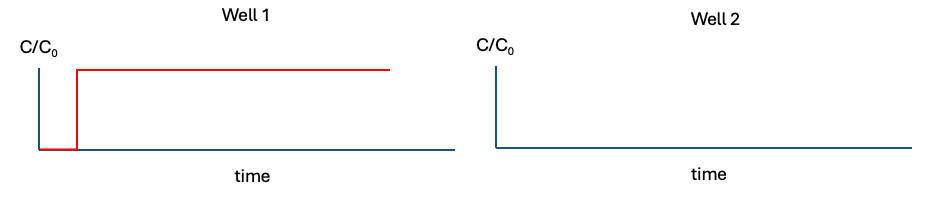
\includegraphics[width=6in]{WellsHistory.png} 
\end{center}
%\caption{}
%\label{fig:aquifer1}
%\end{figure}
\item Constant source with dispersion, no reactions, or decay. ~\\~\\
%\begin{figure}[h!] %  figure placement: here, top, bottom, or page
%\centering
\begin{center}
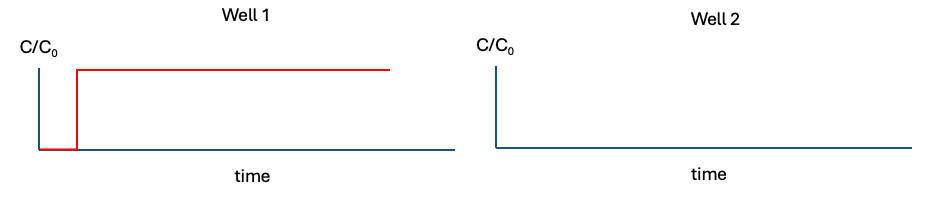
\includegraphics[width=6in]{WellsHistory.png} 
\end{center}
%\caption{}
%\label{fig:aquifer1}
%\end{figure}
\clearpage %%%%%%%%%%%%%%%%%%%%%%%%%%%%
\item Constant source with dispersion, linear equilibrium adsorbtion, but no decay. ~\\~\\
%\begin{figure}[h!] %  figure placement: here, top, bottom, or page
%\centering
\begin{center}
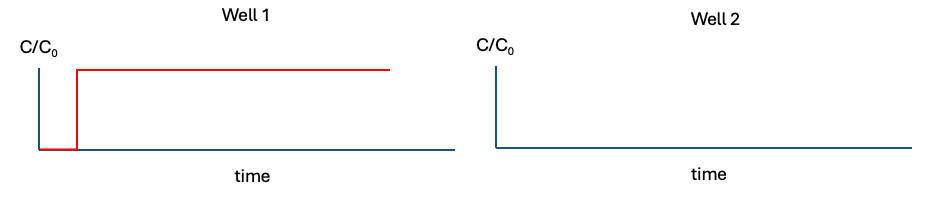
\includegraphics[width=6in]{WellsHistory.png} 
\end{center}
%\caption{}
%\label{fig:aquifer1}
%\end{figure}
\item Constant source with dispersion, linear equilibrium adsorbtion, and 1st-order decay. ~\\~\\
%\begin{figure}[h!] %  figure placement: here, top, bottom, or page
%\centering
\begin{center}
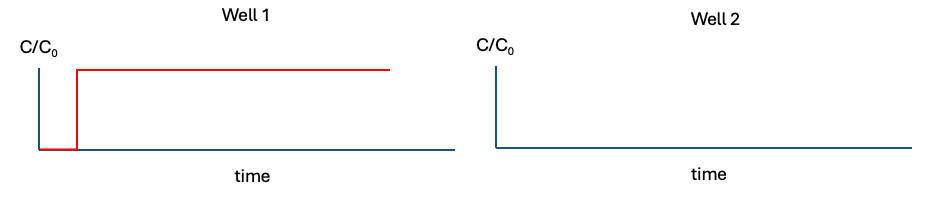
\includegraphics[width=6in]{WellsHistory.png} 
\end{center}
%\caption{}
%\label{fig:aquifer1}
%\end{figure}
\item Finite duration source; no dispersion, reactions, or decay. ~\\~\\
%\begin{figure}[h!] %  figure placement: here, top, bottom, or page
%\centering
\begin{center}
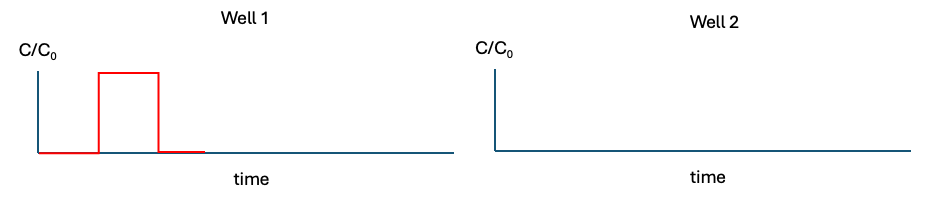
\includegraphics[width=6in]{PulseHistory.png} 
\end{center}
%\caption{}
%\label{fig:aquifer1}
%\end{figure}
\clearpage %%%%%%%%%%%%%%%%%%%%%%%%%%%%%%%%%
\item Finite duration source with dispersion, no reactions, or decay. ~\\~\\
%\begin{figure}[h!] %  figure placement: here, top, bottom, or page
%\centering
\begin{center}
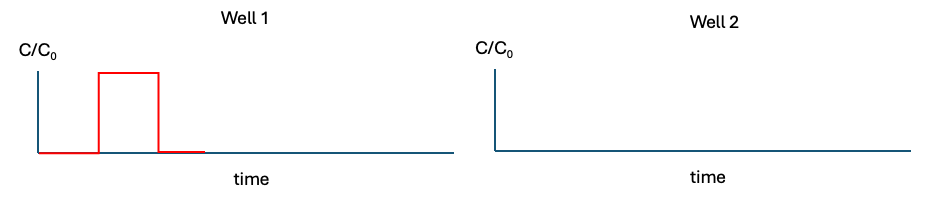
\includegraphics[width=6in]{PulseHistory.png} 
\end{center}
%\caption{}
%\label{fig:aquifer1}
%\end{figure}
\item Finite duration with dispersion, linear equilibrium adsorbtion, but no decay. ~\\~\\
%\begin{figure}[h!] %  figure placement: here, top, bottom, or page
%\centering
\begin{center}
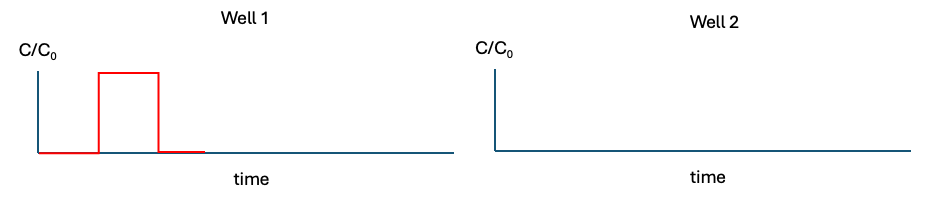
\includegraphics[width=6in]{PulseHistory.png} 
\end{center}
%\caption{}
%\label{fig:aquifer1}
%\end{figure}
\item Finite duration with dispersion, linear equilibrium adsorbtion, and 1st-order decay. ~\\~\\
%\begin{figure}[h!] %  figure placement: here, top, bottom, or page
%\centering
\begin{center}
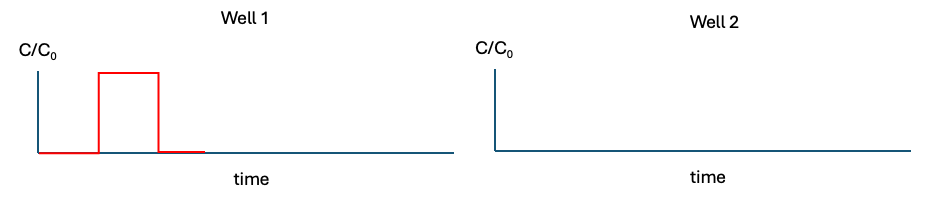
\includegraphics[width=6in]{PulseHistory.png} 
\end{center}
%\caption{}
%\label{fig:aquifer1}
%\end{figure}
\clearpage %%%%%%%%%%%%%%%%%%%%%%%%%%%%%%%%%
\item Declining source with dispersion, no reactions, or decay. ~\\~\\
%\begin{figure}[h!] %  figure placement: here, top, bottom, or page
%\centering
\begin{center}
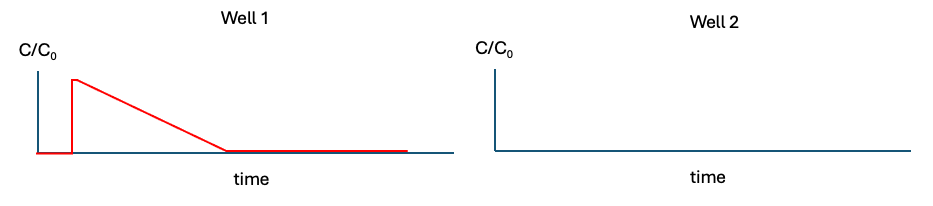
\includegraphics[width=6in]{DeclineHistory.png} 
\end{center}
%\caption{}
%\label{fig:aquifer1}
%\end{figure}
\item Sequence of finite duration sources with dispersion, no reactions, or decay. ~\\~\\
%\begin{figure}[h!] %  figure placement: here, top, bottom, or page
%\centering
\begin{center}
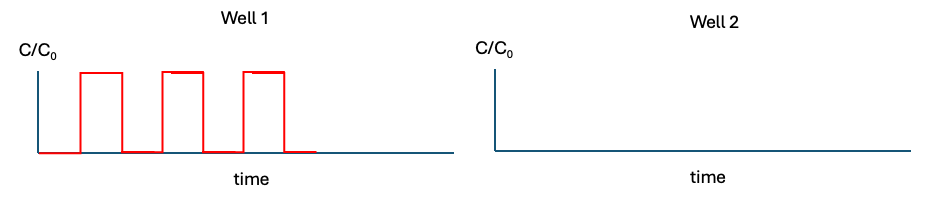
\includegraphics[width=6in]{SequenceHistory.png} 
\end{center}
%\caption{}
%\label{fig:aquifer1}
%\end{figure}
\end{enumerate}
\clearpage %%%%%%%%%%%%%%%%%%%%%%%%%%%%%%%%%
\item Figure \ref{fig:fourtraces} is a plot of concentration histories of constituients introduced into a 1-meter long column at $t=0~minutes$, $x=0~cm$.  Species 1 is known to be conservative and non-reactive (with the aquifer solids).

\begin{figure}[h!] %  figure placement: here, top, bottom, or page
\centering
\begin{center}
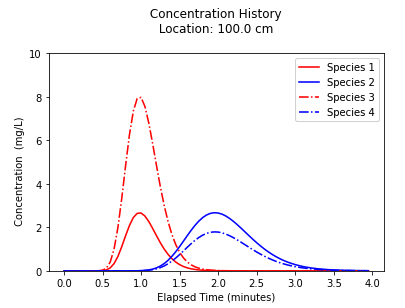
\includegraphics[width=4in]{fourtraces.png} 
\end{center}
\caption{Concentration histories in a porous column}
\label{fig:fourtraces}
\end{figure}


Determine:
\begin{enumerate}[a)]
\item The specific discharge if the porosity is 0.30.
\item The distribution coefficients (assume linear, instantaneous, equilibrium adsorbtion isotherms) for species 2, 3, and 4, if the solids density is $2.97~\frac{g}{cc}$.
\item An estimate of the dispersion coefficient for species 3
\item Predict the concentration history for species 3 at $x=50~cm$
\end{enumerate}
\clearpage %%%%%%%%%%%%%%%%%%%%%%%%%%%%%%%%%
~
\clearpage %%%%%%%%%%%%%%%%%%%%%%%%%%%%%%%%%
\item Figure \ref{fig:schoolyard} is a schematic of a rectangular excavation cut into surface clay for a sewer pipe which was placed, then backfilled with sand. The hydraulic conductivity of the sand is $20.0~\frac{ft}{day}$. The hydraulic gradient in the sand is $0.1$. The porosity of the sand is $0.30$. The longitudinal dispersivity of the sand is $10.0~\frac{ft}{day}$. The sewer leaks and introduces a steady input of water (that causes the hydraulic gradient) located at the access shaft at a concentration of $1000~\frac{mg}{L}$ of some constituient. The consituient has a retardation factor of 2.0.

\begin{figure}[h!] %  figure placement: here, top, bottom, or page
\centering
\begin{center}
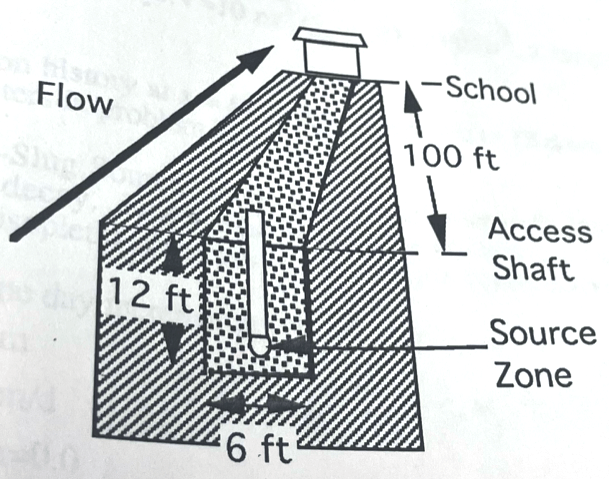
\includegraphics[width=4in]{schoolyard.png} 
\end{center}
\caption{Sewer Pipe Trench near a School}
\label{fig:schoolyard}
\end{figure}

Determine:

The concentration 100 feet away from the release in the sand near the school yard 6,16,25,and 75 days after the leak begins.  
\clearpage %%%%%%%%%%%%%%%%%%%%%%%%%%%%%%%%%
~
\clearpage %%%%%%%%%%%%%%%%%%%%%%%%%%%%%%%%%
\end{enumerate}

\end{document}

